% !TEX root = main.tex

\secmoveup
\section{Introduction}
% \sectextmoveup

%%% para 1: overall challenge of the field
The Internet is home to a large number of images, many of which lack useful
captions. While a growing body of work has developed the capacity to narrate
the contents of generic images~\cite{Donahue2015LongTR, Vinyals2015ShowAT,
Fang2015FromCT, Karpathy2015DeepVA, Rennie2017SelfCriticalST, Lu2017KnowingWT,
Anderson2017BottomUpAT, Cornia2019ShowCT}, these techniques still have two
important weaknesses. The first weakness is in world knowledge. Most captioning
systems are aware of generic object categories but unaware of names and places.
Also generated captions are often inconsistent with commonsense knowledge. The
second weakness is in linguistic expressiveness. The community has observed
that generated captions tend to be shorter and less diverse than human-written
captions~\cite{vinyals2016show,li2018generating}. Most captioning systems rely
on a fixed vocabulary and cannot correctly place or spell new or rare words.
%% use some of these stuff in the next para
\eat{A growing body of work seeks to automatically generate captions that
describe the objects and relationships using only visual cues extracted from
the image itself~\cite{Donahue2015LongTR, Vinyals2015ShowAT, Fang2015FromCT,
Karpathy2015DeepVA, Rennie2017SelfCriticalST, Lu2017KnowingWT,
Anderson2017BottomUpAT, Cornia2019ShowCT}. While generic image descriptions
have their uses, such as for individuals with vision impairments, they are
often of less benefit to the average user. To produce more useful image
captions we need to go beyond generic descriptions and introduce information
that cannot be gleaned directly from the image alone. Fortunately, many images
have an associated context such as a news article, web page, or social media
post, which give the image greater meaning than can be extracted from its
pixels. To generate captions that go beyond generic description and actually
add information that could not be gleaned from the image alone we must take
this context into account. We focus on the news image captioning task in order
to design practical methods for exploiting contextual information. News image
captioning is an interesting instance of contextual captioning where news
articles provide context to images.}

\begin{figure}[t]
	\begin{center}
		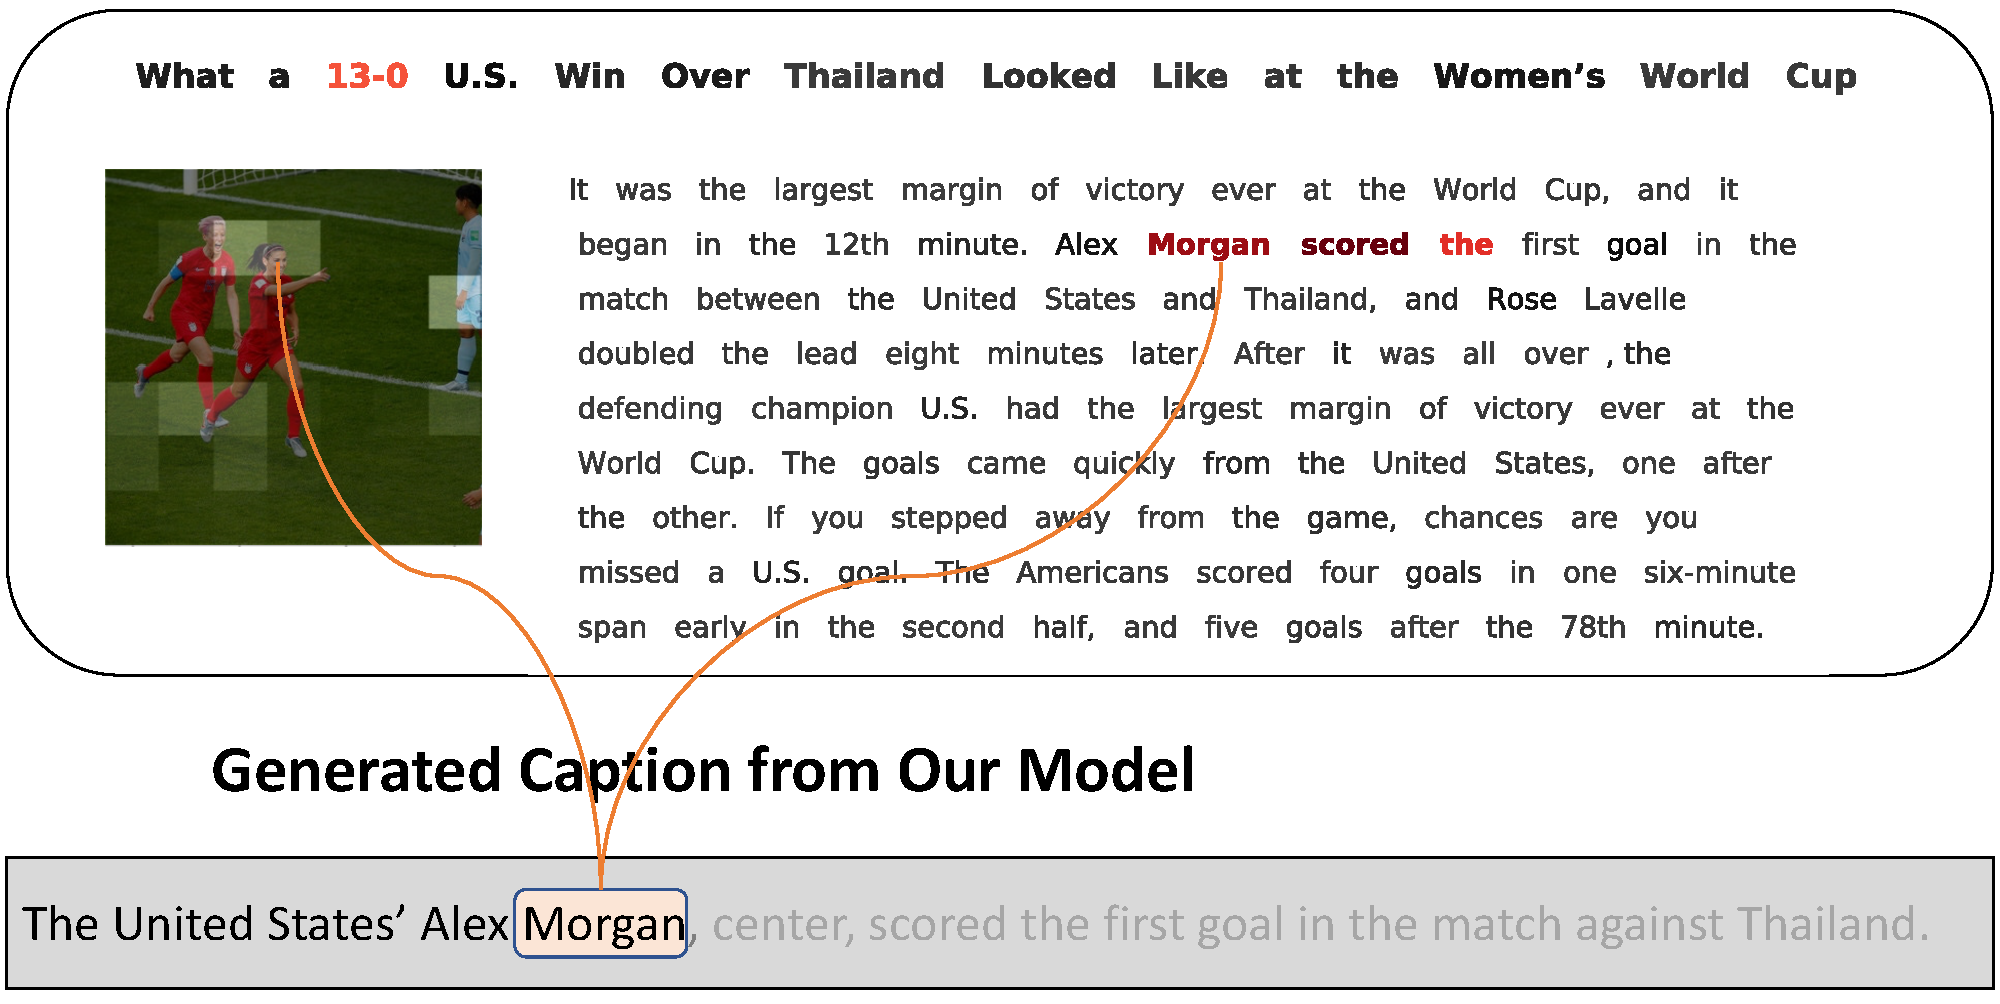
\includegraphics[width=0.99\linewidth]{figures/figure_1.pdf}
	\end{center}
	\capmoveup
   \caption{An example of entity-aware news image captioning. Given a news
	 article and an image (top), our model generates a relevant caption
	 (bottom) by attending over the contexts. Here we show the attention scores
	 over the image patches and the article text as the decoder generates the
	 word ``Morgan". Image patches with higher attention have a lighter shade,
	 while highly-attended words are in red. The orange lines point to
	 the highly attended regions.}
	 \postfigmoveup
	\label{fig:teaser}
\end{figure}

\eat{However, images on the internet are
often associated with a context such as a news article, web page, or social
media post, which give the image greater meaning than can be extracted from its
pixels. To generate captions that go beyond generic description and actually
add information that could not be gleaned from the image alone we must take
this context into account.}

%%% para 2: sepcific challenges of news captions w example
%give the image greater meaning than can be extracted from its pixels.
News image captioning is an interesting case study for tackling these two
challenges. Not only do news captions describe specific people, organizations
and places, but the associated news articles also provide rich contextual
information. The language used in news is evolving, with both the vocabulary
and style changing over time. Thus news captioning approaches need to adapt to
new words and concepts that emerge over a longer period of time (e.g. {\em
walkman} in the 1990s or {\em mp3 player} in the 2000s). Existing
approaches~\cite{Tariq2017ACE,Ramisa2016BreakingNewsAA,Biten2019GoodNews} rely
on text extraction or template filling, which prevents the results from being
linguistically richer than the template generator and are error-prone due to
the difficulty in ranking entities for gap filling. Successful strategies for
news image captioning can be generalized to images from domains
with other types of rich context, such as
web pages, social media posts, and user
comments.

\eat{Captions for news images, such as the example in Figure~\ref{fig:teaser},
typically contain details which cannot be derived from the image alone. They
also frequently contain proper nouns such as names of people, places, and
organizations -- in many cases these proper nouns are rare (most people and
places do not have many news articles written about them). A system capable of
generating high quality news captions should therefor make extensive use of the
provided context and be tuned for generating rare proper nouns. Existing
approaches to news image captioning~\cite{Tariq2017ACE,
Ramisa2016BreakingNewsAA,
	Biten2019GoodNews}  rely on text extraction or
template filling to deal with rare contextual terms such as names of people and
organizations. This makes them relatively inflexibility and means they cannot
be trained end-to-end. Moreover, existing approaches do not include specialized
visual models for frequent nouns -- experiments on the MSCOCO dataset have
shown
that pre-trained object detectors tuned for frequent nouns
lead to more accurate captions~\cite{Wu2016HighLevel,Gan2017Semantic}.}


\eat{The contextual word
	embeddings provided by these methods have helped establish new
	state-of-the-art
	results on many natural language understanding benchmarks including GLUE
	\cite{Wang2019GLUE}, SuperGLUE~\cite{Wang2019SuperGLUEAS}, and SQuAD
	\cite{Rajpurkar2016SQuAD, Rajpurkar2018KnowWY}, even surpassing the human
	baselines in many cases.}

\eat{In parallel to the development of these pre-training methods, many novel
techniques have been proposed to improve training convergence and handle more
diverse data inputs. The most significant contribution is the use of byte-pair
encoding (BPE)~\cite{Sennrich2015NeuralMT} to represent a rare word as a
sequence of subword units, thus giving models the ability to handle an open
vocabulary.}

\eat{that 1) combines specialized modules for
incorporating and selectively attending to image features, human faces, and
news article text and 2) applies a state-of-the-art sequence generation model
which is able to generate rare tokens, such as proper names, even when they do
not form part of the training data. Our model relies on a }

We propose an end-to-end model for news image captioning with a novel
combination of sequence-to-sequence neural networks, language representation
learning, and vision subsystems. In particular, we address the knowledge gap by
computing multi-head attention on the words in the article, along with faces
and objects that are extracted from the image. We address the linguistic gap
with a flexible byte-pair-encoding that can generate unseen words. We use
dynamic convolutions and mix different linguistic representation layers to make
the neural network representation richer. We also propose a new dataset,
NYTimes800k, that is 70\% larger than GoodNews~\cite{Biten2019GoodNews} and has
higher-quality articles along with additional image location information. We
observe a performance gain of $6.8\times$ in BLEU-4 ($0.89 \rightarrow 6.05$)
and $4.1\times$ in CIDEr ($13.1 \rightarrow 53.8$) compared to previous
work~\cite{Biten2019GoodNews}. On both datasets we observe consistent gains for
each new component in our language, vision, and knowledge-aware system. We also
find that our model generates names not seen during training, resulting in
linguistically richer captions, which are closer in length (mean 15 words) to
the ground truth (mean 18 words) than the previous state of the art (mean 10
words).

% with the average caption containing 15 words, which is
%longer than the baseline~\cite{Biten2019GoodNews} (10 words) and a lot closer
%to the ground-truth length (18 words).

%6.22/0.89
%60.6/13.1
%The key components of our approach are selectively attending to different
%aspects of the two modalities: image
%regions, faces, and text sequences.
%Using powerful pre-trained contextual language models to represent news
%articles -- allowing articles with text not see during training  tuples
%required for training.
%Using sub-word units, which when combined with pre-training, allow for the
%generation of tokens not seen during training.


%\sout{
%Most existing captioning systems can only generate a generic description
%of an
%image~\cite{Donahue2015LongTR, Vinyals2015ShowAT, Fang2015FromCT,
%Karpathy2015DeepVA, Rennie2017SelfCriticalST, Lu2017KnowingWT,
%Anderson2017BottomUpAT, Cornia2019ShowCT}, mainly because these architectures
%cannot handle an open vocabulary and early captioning datasets such as MS COCO
%\cite{Lin2014MicrosoftCC, Chen2015MicrosoftCC} and Flickr30k
%\cite{Young2014FromID} were annotated using only visual cues present in the
%image. More recently, datasets such as TIME~\cite{Tariq2017ACE}, BreakingNews
%\cite{Ramisa2016BreakingNewsAA}, and GoodNews~\cite{Biten2019GoodNews} include
%real-life captions written by professional journalists. However, existing
%models that are trained on these news datasets still need to rely on either
%extractive methods or templates to insert named entities.}

Our main contributions include:

\begin{enumerate}
	\itemsep0em
   \item A new captioning model that incorporates transformers, an
   attention-centric language model, byte-pair encoding, and attention over
   four different modalities (text, images, faces, and objects). \eat{We show
   that our model achieves state-of-the-art results with a significant margin
   over previous methods, and }

   \item Significant performance gains over all metrics, with associated
   ablation studies quantifying the contributions of our main modeling
   components using BLEU-4, CIDEr, precision \& recall of named entities and
   rare proper nouns, and linguistic quality metrics.

	\item NYTimes800k, the largest news image captioning dataset to date,
	containing 445K articles and 793K images with captions from The New York
	Times spanning 14 years. NYTimes800k builds and improves upon the recently
	proposed GoodNews dataset~\cite{Biten2019GoodNews}. It has 70\% more
	articles and includes image locations within the article text. The dataset,
	code, and pre-trained models are available on
	GitHub\footnote{\href{https://github.com/alasdairtran/transform-and-tell}{https://github.com/alasdairtran/transform-and-tell}}.
\end{enumerate}
